\section{Museum's role in society}

In the recommendation letter report \emph{“Museums in the society - trust, things and time,”} the standing committee of Cultural Affairs presents the overall political direction for Norwegian museum policy towards the year 2050 (Figure 1.1). The report establishes that Norwegian museum institutions take aim to express both historical and current developments in society. And that museum institutions play an important role in our own time’s understanding of ourselves - both who we have been, who we are, and whom we want to be \autocite[p. 7]{melding23}. Modern museum operations aim to actively turn to the general public with the objective to build and share knowledge, increase enlightenment and cultivate cultural capital. Where the early museum institutions, first and foremost, were accessible to a small number of privileged class members, it is now expected that museums purposefully reach out to be open and accessible to all residents and age groups \autocite[p. 14]{melding23}. In Norway, museums are increasingly understood as both knowledge and social institutions, where dissemination and exhibition practice are curated accordingly. At the same time, museums have emerged as an alternative learning arena for school children, first regarding history teaching, but later in many other subject areas as well. In a society where polarization and public debate are intensifying, arenas that have the public's confidence in being able to nuance and disseminate different perspectives are needed \autocite[p. 7]{melding23}.

\begin{figure}[H]
\centering
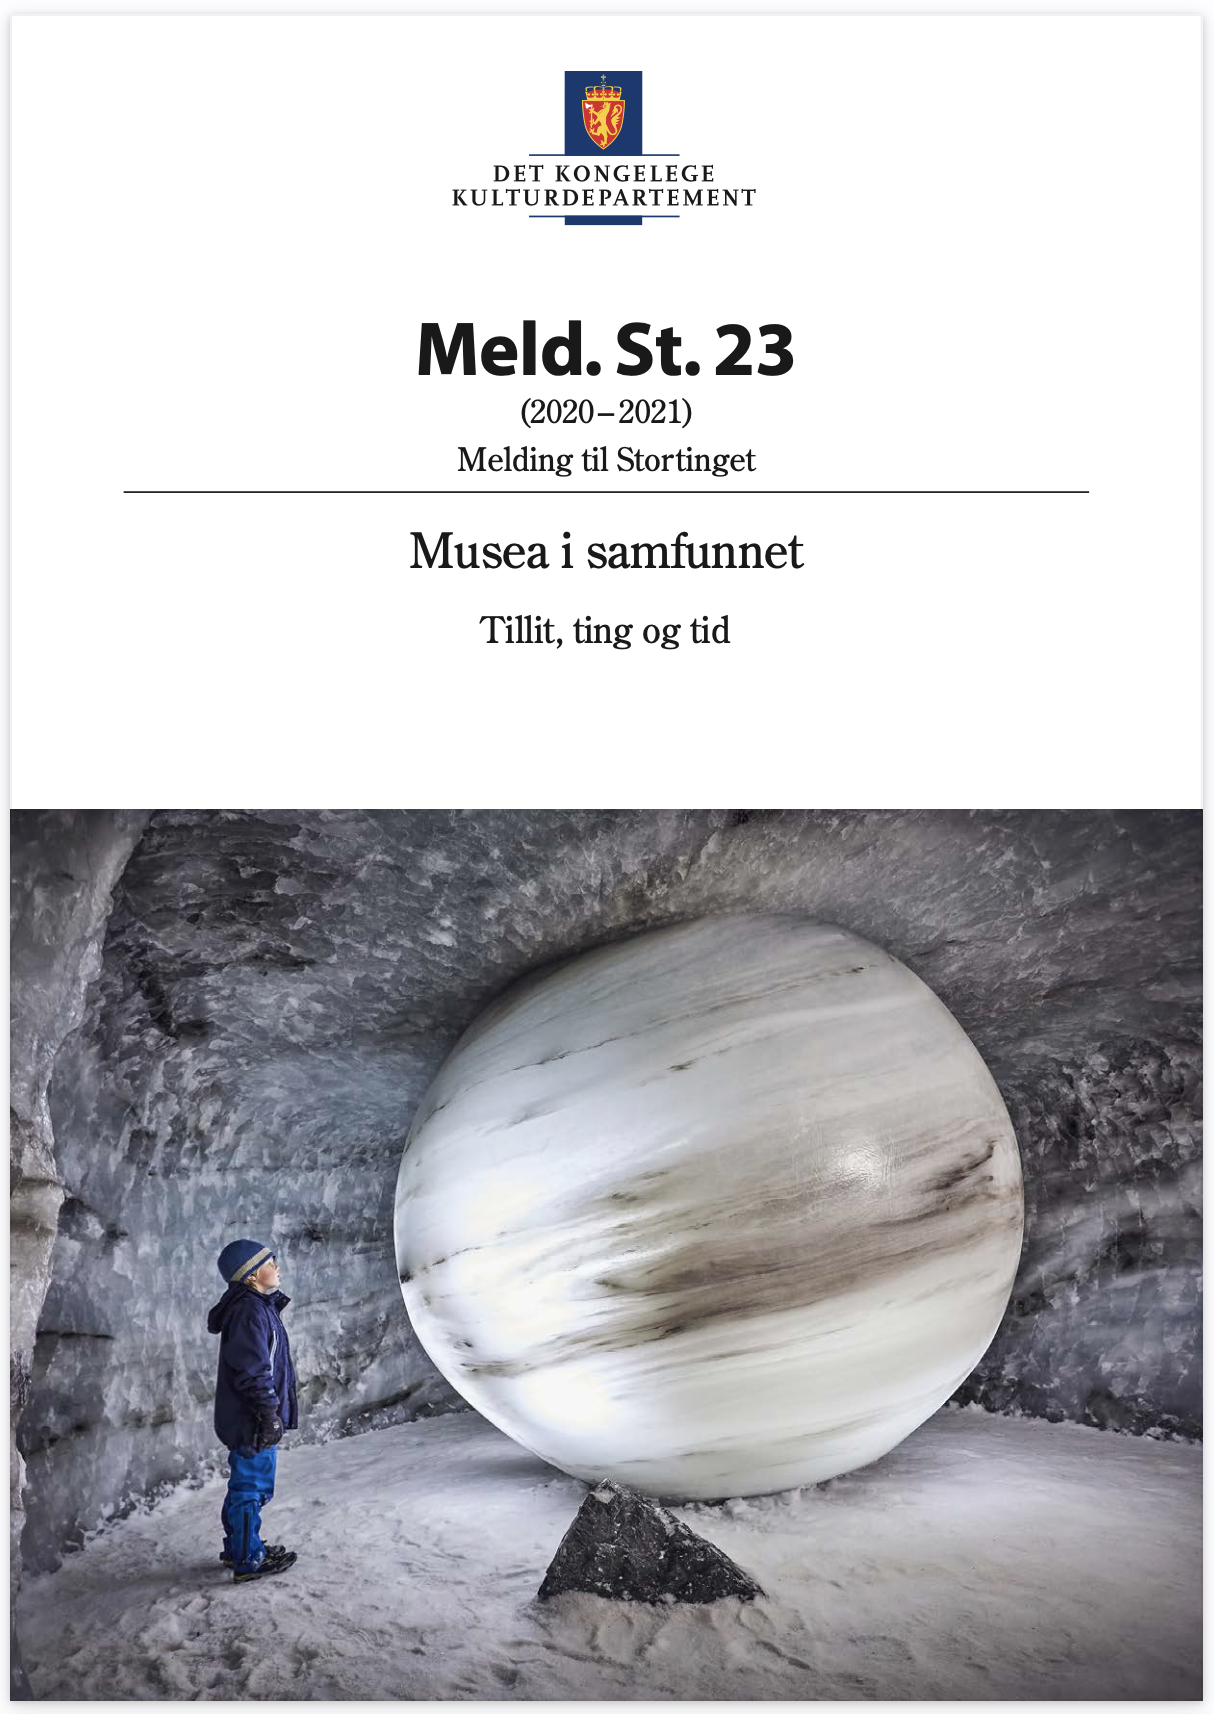
\includegraphics[width=8cm]{pictures/Introduction/stortingsmelding_hoykant.png}
\caption{The recommendation letter report Meld.St.23 \emph{“Museums in the society - trust, things and time"}}
\end{figure}

There is a saying among historians that \emph{"the past teaches us about the present"}. History is a subject that is extra rich in perspectives, explanations, and ideas about how people have lived, thought, and acted. It positions us to see patterns that might otherwise be invisible in the present – thus providing a crucial perspective for understanding and solving current and future problems \autocite{UW_website}. Being a knowledge institution, museums have the power to both define and showcase relevant historical events as a perspective to inform present societal issues and debates. 

% Klimahistorie: eget avsnitt?

% Skiftet til museene handler ikke bare om å fornye seg, altså appellere til en bredere målgruppe, men det handler om å "henge med i tiden", og klare å forankre dagsaktuelle debatter/ samtaler med et faglig, vitenskapelig korrekt, blikk.

\section{Research Question/ Framing}
The aim of this study is to gain insight to try answer how one can design interactive meaningful experiences in a museum space that addresses sustainability. To understand this, several installations have been analysed as a way to objectify \emph{meaningfulness} as a quality that you can design for. Meaningfulness is generally defined/understood as (...), but this thesis fills a gap where the term is explored through a museum context, adding to existing literature on future museum design by using sustainability as a topic representing a contemporary discourse addressed in museum spaces.

This thesis aim to answer how one can design meaningful interactive experiences in a museum space that addresses sustainability. This is attempted through objectifying meaningfulness as a quality that you can design for in a museum, by identifying and analysing dialogic relations between visitor and installation.

\section{Scientific contribution}
The thesis investigates how interactivity can support visitors meaning-making in a museum space. The hypothesis is that an interactive installation or experience have the potential to reinforce the message conveyed in a manner that give rise to thought-provoking or significant reflections that last long after the museum visit. Something which also encompass the power to deliberately stimulate visitors lifestyle choices or actions after the museum visit, in compliance with the museums agenda and vision. Special attention has been given to museums that aims to encourage social action, like climate consciousness or climate action.
One theoretical and one practical.

\section{About the structure of thesis}
The thesis is divided into three parts; Introduction, Design Process, and Review/ Evaluation. The (report) structure reflects the methodological nature of doing Research through Design, where the Design Process is evidence of the practical activities shaping the thesis project. If not referenced otherwise, all pictures in this thesis come from a shared photo library the research buddies and I have built up and accumulated during fieldwork. The same goes for illustrations. If not referenced else-wise, they are illustrated by me.

\subsubsection{Chapter 2}
Chapter 2 is a focused selection of terminology and concepts attained from the literature review that has been conducted throughout/during the thesis project. It is structured in the hope that designers interested in the topic can adopt the concepts as a vocabulary and mean of understanding some of what goes on in the museum world. The literature review has nonetheless been crucial for the thesis evolution. On the one hand, it has influenced the research framing and interest, shaped and refined the research question, and leveraged the vocabulary when documenting/ recounting an exhibition- and installation experience. While on the other hand, it has influenced the convergent and divergent thought process when going in and out/back-and-forth of practical and theoretical work, the designer role, and the researcher role.

% The next three chapters differs from chapter 2 because of their direct and practical application. Shaping the rest of the thesis and used for critiquing of the exhibitions/ installations.

\subsubsection{Chapter 3}
The next three chapters is a continuation of the literature review. Where Chapter 2 indirectly affect the thesis evolution, Chapter 3, 4 and 5 present three theoretical frameworks that have practically/directly guided e.g. data-gathering guides during fieldwork, both for observations, interviews and analytical critique. In addition to this, in chapter 6, we build upon and borrow concepts in the making of an analytical tool, my proposal as a new way of designing for meaningfulness.

\begin{itemize}
    \item Chapter 3: Hybrid place
    \item Chapter 4: Place as a dialogue
    \item Chapter 5: Sense-making
    \item Chapter 6: A new way to design for meaningfulness?
\end{itemize}
\par


The use of theory is essential to any academic discipline. Before we embark on to the Theory chapters, it is necessary to go into how theory have been put to use throughout the thesis project. In my attempt to answer how one can design meaningful interactive experiences in a museum space that addresses sustainability, I have chosen to look into three theoretical frameworks that give the means to understand interactive artefacts dialogic qualities - as an answer to how museum spaces can look at their respective installations and judge whether or not they stimulate the visitor to dialogue (conversations). The hypothesis is that there lies value for the museum to judge whether or not their installations promote dialogue. 
